\documentclass[11pt,addpoints,answers]{exam}

%%%%%%%%%%%%%%%%%%%%%%%%%%%%%%%%%%%%%%%%%%%
% Commands for customizing the assignment %
%%%%%%%%%%%%%%%%%%%%%%%%%%%%%%%%%%%%%%%%%%%

\newcommand{\courseNum}{10-423/10-623}
\newcommand{\courseName}{Generative AI}
\newcommand{\courseSem}{Spring 2024}
\newcommand{\courseUrl}{\url{http://423.mlcourse.org}}
\newcommand{\hwNum}{Homework 0}
\newcommand{\hwTopic}{PyTorch Primer}
\newcommand{\hwName}{\hwNum: \hwTopic}
\newcommand{\outDate}{Aug. 28, 2024}
\newcommand{\dueDate}{Sep. 9, 2024}
\newcommand{\taNames}{Haoyang, Afreen, Katie, Ketan, Ryan, Shrikara, and Jacob}
\newcommand{\homeworktype}{\string written+prog}
\newcommand{\overleafUrl}{}

%% To HIDE SOLUTIONS (to post at the website for students), set this value to 0: \def\issoln{0}
\providecommand{\issoln}{0}
%\providecommand{\issoln}{1}

%-----------------------------------------------------------------------------
% PACKAGES AND OTHER DOCUMENT CONFIGURATIONS
%-----------------------------------------------------------------------------

\usepackage[margin=1in]{geometry}
\usepackage{amsmath, amsfonts}
\usepackage{enumerate}
\usepackage{graphicx}
\usepackage{titling}
\usepackage{url}
\usepackage{xfrac}
\usepackage{natbib}
\usepackage{amssymb}
\usepackage{amsthm}
\usepackage{paralist}
\usepackage{epstopdf}
\usepackage{tabularx}
\usepackage{longtable}
\usepackage{multirow}
\usepackage{multicol}
\usepackage[colorlinks=true,urlcolor=blue]{hyperref}
\usepackage{algorithm}
\usepackage{algorithmicx}
\usepackage[noend]{algpseudocode}
\usepackage{float}
\usepackage{enumerate}
\usepackage{array}
\usepackage{environ}
\usepackage{times}
\usepackage{textcomp}
\usepackage{caption}
\usepackage{parskip} % For NIPS style paragraphs.
\usepackage[compact]{titlesec} % Less whitespace around titles
\usepackage[inline]{enumitem} % For inline enumerate* and itemize*
\usepackage{datetime}
\usepackage{comment}
% \usepackage{minted}
\usepackage{lastpage}
\usepackage{color}
% \usepackage{xcolor}
\usepackage[dvipsnames]{xcolor}
\usepackage[final]{listings}
\usepackage{tikz}
\usetikzlibrary{shapes,decorations}
\usepackage{framed}
\usepackage{booktabs}
\usepackage{cprotect}
\usepackage{verbatimbox}
\usepackage{multicol}
\usepackage{hyperref}
\usepackage{subcaption}
\usepackage{mathtools} % For drcases
\usepackage{cancel}
\usepackage[many]{tcolorbox}
\usepackage{soul}
\usepackage[bottom]{footmisc}
\usepackage{bm}
\usepackage{wasysym}
\usepackage{lipsum}

\usepackage{tikz}
\usetikzlibrary{arrows}
\usetikzlibrary{arrows.meta}
\usetikzlibrary{shapes.geometric}
\usetikzlibrary{positioning, arrows, automata, calc}
\usepackage{transparent}
\usepackage{tikz-cd}

%%%%%%%%%%%%%%%%%%%%%%%%%%%%%%%%%%%%%%%%%%%
% Formatting for \CorrectChoice of "exam" %
%%%%%%%%%%%%%%%%%%%%%%%%%%%%%%%%%%%%%%%%%%%

\CorrectChoiceEmphasis{}
\checkedchar{\blackcircle}

\newenvironment{checkboxessquare}{
    \begingroup
    \checkboxchar{$\Box$} \checkedchar{$\blacksquare$} % change checkbox style locally
    \begin{checkboxes}
    }{
    \end{checkboxes}
    \endgroup
    }

%%%%%%%%%%%%%%%%%%%%%%%%%%%%%%%%%%%%%%%%%%%
% Better numbering                        %
%%%%%%%%%%%%%%%%%%%%%%%%%%%%%%%%%%%%%%%%%%%

% \numberwithin{equation}{section} % Number equations within sections (i.e. 1.1, 1.2, 2.1, 2.2 instead of 1, 2, 3, 4)
% \numberwithin{figure}{section} % Number figures within sections (i.e. 1.1, 1.2, 2.1, 2.2 instead of 1, 2, 3, 4)
% \numberwithin{table}{section} % Number tables within sections (i.e. 1.1, 1.2, 2.1, 2.2 instead of 1, 2, 3, 4)

%%%%%%%%%%%%%%%%%%%%%%%%%%%%%%%%%%%%%%%%%%
% Custom commands                        %
%%%%%%%%%%%%%%%%%%%%%%%%%%%%%%%%%%%%%%%%%%
\newcommand{\blackcircle}{\tikz\draw[black,fill=black] (0,0) circle (1ex);}
\renewcommand{\circle}{\tikz\draw[black] (0,0) circle (1ex);}

\newcommand{\solo}{ \textcolor{orange}{[SOLO]} }
\newcommand{\open}{ \textcolor{blue}{[OPEN]} }


%%%%%%%%%%%%%%%%%%%%%%%%%%%%%%%%%%%%%%%%%%
% Custom commands for Math               %
%%%%%%%%%%%%%%%%%%%%%%%%%%%%%%%%%%%%%%%%%%
\newcommand{\vc}[1]{\boldsymbol{#1}}
\newcommand{\adj}[1]{\frac{\partial \ell}{\partial #1}}
\newcommand{\chain}[2]{\adj{#2} = \adj{#1}\frac{\partial #1}{\partial #2}}
\newcommand{\ntset}{test}
\newcommand{\zerov}{\mathbf{0}}
\DeclareMathOperator*{\argmin}{argmin}

% mathcal
\newcommand{\Ac}{\mathcal{A}}
\newcommand{\Bc}{\mathcal{B}}
\newcommand{\Cc}{\mathcal{C}}
\newcommand{\Dc}{\mathcal{D}}
\newcommand{\Ec}{\mathcal{E}}
\newcommand{\Fc}{\mathcal{F}}
\newcommand{\Gc}{\mathcal{G}}
\newcommand{\Hc}{\mathcal{H}}
\newcommand{\Ic}{\mathcal{I}}
\newcommand{\Jc}{\mathcal{J}}
\newcommand{\Kc}{\mathcal{K}}
\newcommand{\Lc}{\mathcal{L}}
\newcommand{\Mc}{\mathcal{M}}
\newcommand{\Nc}{\mathcal{N}}
\newcommand{\Oc}{\mathcal{O}}
\newcommand{\Pc}{\mathcal{P}}
\newcommand{\Qc}{\mathcal{Q}}
\newcommand{\Rc}{\mathcal{R}}
\newcommand{\Sc}{\mathcal{S}}
\newcommand{\Tc}{\mathcal{T}}
\newcommand{\Uc}{\mathcal{U}}
\newcommand{\Vc}{\mathcal{V}}
\newcommand{\Wc}{\mathcal{W}}
\newcommand{\Xc}{\mathcal{X}}
\newcommand{\Yc}{\mathcal{Y}}
\newcommand{\Zc}{\mathcal{Z}}

% mathbb
\newcommand{\Ab}{\mathbb{A}}
\newcommand{\Bb}{\mathbb{B}}
\newcommand{\Cb}{\mathbb{C}}
\newcommand{\Db}{\mathbb{D}}
\newcommand{\Eb}{\mathbb{E}}
\newcommand{\Fb}{\mathbb{F}}
\newcommand{\Gb}{\mathbb{G}}
\newcommand{\Hb}{\mathbb{H}}
\newcommand{\Ib}{\mathbb{I}}
\newcommand{\Jb}{\mathbb{J}}
\newcommand{\Kb}{\mathbb{K}}
\newcommand{\Lb}{\mathbb{L}}
\newcommand{\Mb}{\mathbb{M}}
\newcommand{\Nb}{\mathbb{N}}
\newcommand{\Ob}{\mathbb{O}}
\newcommand{\Pb}{\mathbb{P}}
\newcommand{\Qb}{\mathbb{Q}}
\newcommand{\Rb}{\mathbb{R}}
\newcommand{\Sb}{\mathbb{S}}
\newcommand{\Tb}{\mathbb{T}}
\newcommand{\Ub}{\mathbb{U}}
\newcommand{\Vb}{\mathbb{V}}
\newcommand{\Wb}{\mathbb{W}}
\newcommand{\Xb}{\mathbb{X}}
\newcommand{\Yb}{\mathbb{Y}}
\newcommand{\Zb}{\mathbb{Z}}

% mathbf lowercase
\newcommand{\av}{\mathbf{a}}
\newcommand{\bv}{\mathbf{b}}
\newcommand{\cv}{\mathbf{c}}
\newcommand{\dv}{\mathbf{d}}
\newcommand{\ev}{\mathbf{e}}
\newcommand{\fv}{\mathbf{f}}
\newcommand{\gv}{\mathbf{g}}
\newcommand{\hv}{\mathbf{h}}
\newcommand{\iv}{\mathbf{i}}
\newcommand{\jv}{\mathbf{j}}
\newcommand{\kv}{\mathbf{k}}
\newcommand{\lv}{\mathbf{l}}
\newcommand{\mv}{\mathbf{m}}
\newcommand{\nv}{\mathbf{n}}
\newcommand{\ov}{\mathbf{o}}
\newcommand{\pv}{\mathbf{p}}
\newcommand{\qv}{\mathbf{q}}
\newcommand{\rv}{\mathbf{r}}
\newcommand{\sv}{\mathbf{s}}
\newcommand{\tv}{\mathbf{t}}
\newcommand{\uv}{\mathbf{u}}
\newcommand{\vv}{\mathbf{v}}
\newcommand{\wv}{\mathbf{w}}
\newcommand{\xv}{\mathbf{x}}
\newcommand{\yv}{\mathbf{y}}
\newcommand{\zv}{\mathbf{z}}

% mathbf uppercase
\newcommand{\Av}{\mathbf{A}}
\newcommand{\Bv}{\mathbf{B}}
\newcommand{\Cv}{\mathbf{C}}
\newcommand{\Dv}{\mathbf{D}}
\newcommand{\Ev}{\mathbf{E}}
\newcommand{\Fv}{\mathbf{F}}
\newcommand{\Gv}{\mathbf{G}}
\newcommand{\Hv}{\mathbf{H}}
\newcommand{\Iv}{\mathbf{I}}
\newcommand{\Jv}{\mathbf{J}}
\newcommand{\Kv}{\mathbf{K}}
\newcommand{\Lv}{\mathbf{L}}
\newcommand{\Mv}{\mathbf{M}}
\newcommand{\Nv}{\mathbf{N}}
\newcommand{\Ov}{\mathbf{O}}
\newcommand{\Pv}{\mathbf{P}}
\newcommand{\Qv}{\mathbf{Q}}
\newcommand{\Rv}{\mathbf{R}}
\newcommand{\Sv}{\mathbf{S}}
\newcommand{\Tv}{\mathbf{T}}
\newcommand{\Uv}{\mathbf{U}}
\newcommand{\Vv}{\mathbf{V}}
\newcommand{\Wv}{\mathbf{W}}
\newcommand{\Xv}{\mathbf{X}}
\newcommand{\Yv}{\mathbf{Y}}
\newcommand{\Zv}{\mathbf{Z}}

% bold greek lowercase
\newcommand{\alphav     }{\boldsymbol \alpha     }
\newcommand{\betav      }{\boldsymbol \beta      }
\newcommand{\gammav     }{\boldsymbol \gamma     }
\newcommand{\deltav     }{\boldsymbol \delta     }
\newcommand{\epsilonv   }{\boldsymbol \epsilon   }
\newcommand{\varepsilonv}{\boldsymbol \varepsilon}
\newcommand{\zetav      }{\boldsymbol \zeta      }
\newcommand{\etav       }{\boldsymbol \eta       }
\newcommand{\thetav     }{\boldsymbol \theta     }
\newcommand{\varthetav  }{\boldsymbol \vartheta  }
\newcommand{\iotav      }{\boldsymbol \iota      }
\newcommand{\kappav     }{\boldsymbol \kappa     }
\newcommand{\varkappav  }{\boldsymbol \varkappa  }
\newcommand{\lambdav    }{\boldsymbol \lambda    }
\newcommand{\muv        }{\boldsymbol \mu        }
\newcommand{\nuv        }{\boldsymbol \nu        }
\newcommand{\xiv        }{\boldsymbol \xi        }
\newcommand{\omicronv   }{\boldsymbol \omicron   }
\newcommand{\piv        }{\boldsymbol \pi        }
\newcommand{\varpiv     }{\boldsymbol \varpi     }
\newcommand{\rhov       }{\boldsymbol \rho       }
\newcommand{\varrhov    }{\boldsymbol \varrho    }
\newcommand{\sigmav     }{\boldsymbol \sigma     }
\newcommand{\varsigmav  }{\boldsymbol \varsigma  }
\newcommand{\tauv       }{\boldsymbol \tau       }
\newcommand{\upsilonv   }{\boldsymbol \upsilon   }
\newcommand{\phiv       }{\boldsymbol \phi       }
\newcommand{\varphiv    }{\boldsymbol \varphi    }
\newcommand{\chiv       }{\boldsymbol \chi       }
\newcommand{\psiv       }{\boldsymbol \psi       }
\newcommand{\omegav     }{\boldsymbol \omega     }

% bold greek uppercase
\newcommand{\Gammav     }{\boldsymbol \Gamma     }
\newcommand{\Deltav     }{\boldsymbol \Delta     }
\newcommand{\Thetav     }{\boldsymbol \Theta     }
\newcommand{\Lambdav    }{\boldsymbol \Lambda    }
\newcommand{\Xiv        }{\boldsymbol \Xi        }
\newcommand{\Piv        }{\boldsymbol \Pi        }
\newcommand{\Sigmav     }{\boldsymbol \Sigma     }
\newcommand{\Upsilonv   }{\boldsymbol \Upsilon   }
\newcommand{\Phiv       }{\boldsymbol \Phi       }
\newcommand{\Psiv       }{\boldsymbol \Psi       }
\newcommand{\Omegav     }{\boldsymbol \Omega     }

%%%%%%%%%%%%%%%%%%%%%%%%%%%%%%%%%%%%%%%%%%%
% Code highlighting with listings         %
%%%%%%%%%%%%%%%%%%%%%%%%%%%%%%%%%%%%%%%%%%%

\definecolor{bluekeywords}{rgb}{0.13,0.13,1}
\definecolor{greencomments}{rgb}{0,0.5,0}
\definecolor{redstrings}{rgb}{0.9,0,0}
\definecolor{light-gray}{gray}{0.95}

\newcommand{\MYhref}[3][blue]{\href{#2}{\color{#1}{#3}}}%

\definecolor{dkgreen}{rgb}{0,0.6,0}
\definecolor{gray}{rgb}{0.5,0.5,0.5}
\definecolor{mauve}{rgb}{0.58,0,0.82}

\lstdefinelanguage{Shell}{
  keywords={tar, cd, make},
  %keywordstyle=\color{bluekeywords}\bfseries,
  alsoletter={+},
  ndkeywords={python3, python, py, javac, java, gcc, c, g++, cpp, .txt, octave, m, .tar},
  %ndkeywordstyle=\color{bluekeywords}\bfseries,
  identifierstyle=\color{black},
  sensitive=false,
  comment=[l]{//},
  morecomment=[s]{/*}{*/},
  commentstyle=\color{purple}\ttfamily,
  %stringstyle=\color{red}\ttfamily,
  morestring=[b]',
  morestring=[b]",
  backgroundcolor = \color{light-gray}
}

\lstset{columns=fixed, basicstyle=\ttfamily,
    backgroundcolor=\color{light-gray},xleftmargin=0.5cm,frame=tlbr,framesep=4pt,framerule=0pt}

\newcommand{\emptysquare}{{\LARGE $\square$}\ \ }
\newcommand{\filledsquare}{{\LARGE $\boxtimes$}\ \ }
\def \ifempty#1{\def\temp{#1} \ifx\temp\empty }


% \newcommand{\squaresolutionspace}[2][\emptysquare]{\newline #1}{#2}
\def \squaresolutionspace#1{ \ifempty{#1} \emptysquare \else #1\hspace{0.75pt}\fi}


\newcommand{\emptycircle}{{\LARGE $\fullmoon$}\ \ }
\newcommand{\filledcircle}{{\LARGE $\newmoon$}\ \ }
\def \circlesolutionspace#1{ \ifempty{#1} \emptycircle \else #1\hspace{0.75pt}\fi}
%%%%%%%%%%%%%%%%%%%%%%%%%%%%%%%%%%%%%%%%%%%
% Custom box for highlights               %
%%%%%%%%%%%%%%%%%%%%%%%%%%%%%%%%%%%%%%%%%%%

% Define box and box title style
\tikzstyle{mybox} = [fill=blue!10, very thick,
    rectangle, rounded corners, inner sep=1em, inner ysep=1em]

% \newcommand{\notebox}[1]{
% \begin{tikzpicture}
% \node [mybox] (box){%
%     \begin{minipage}{\textwidth}
%     #1
%     \end{minipage}
% };
% \end{tikzpicture}%
% }

\NewEnviron{notebox}{

\begin{tikzpicture}
\node [mybox] (box){
    \begin{minipage}{0.95\textwidth}
        \BODY
    \end{minipage}
};
\end{tikzpicture}
}

%%%%%%%%%%%%%%%%%%%%%%%%%%%%%%%%%%%%%%%%%%%
% Commands showing / hiding solutions     %
%%%%%%%%%%%%%%%%%%%%%%%%%%%%%%%%%%%%%%%%%%%
\newcommand{\solutionspace}[4]{\fbox{\begin{minipage}[t][#1][t]{#2} \textbf{#3} \solution{}{#4} \end{minipage}}}

% To HIDE SOLUTIONS, set this value to 0:
%\providecommand{\issoln}{0}
%\providecommand{\issoln}{1}

\ifthenelse{\equal{\issoln}{1}}{

% SOLUTION environment
\newenvironment{soln}{\leavevmode\color{red}\ignorespaces }{}

% QUESTION AUTHORS environment
\newenvironment{qauthor}{\leavevmode\color{blue}\ignorespaces }{}

% Question tester comment environment
\newenvironment{qtester}{\leavevmode\color{green}\ignorespaces}{}

% Question learning objective comment environment
\newenvironment{qlearningobjective}{\leavevmode\color{green}\ignorespaces}{}

}{ % ELSE

  \NewEnviron{soln}{}
  \NewEnviron{qauthor}{}
  \NewEnviron{qtester}{}
  \NewEnviron{qlearningobjective}{}

}

%% To HIDE TAGS set this value to 0:
\def\showtags{0}
%%%%%%%%%%%%%%%%
\ifcsname showtags\endcsname \else \def\showtags{1} \fi
% Default to an empty tags environ.
\NewEnviron{tags}{}{}
\if\showtags 1
% Otherwise, include solutions as below.
\RenewEnviron{tags}{
    \fbox{
    \leavevmode\color{blue}\ignorespaces
    \textbf{TAGS:} \texttt{\url{\BODY}}
    }
    \vspace{-.5em}
}{}
\fi

\newtcolorbox[]{answer_box}[1][]{
    % breakable,
    fit,
    enhanced,
    % nobeforeafter,
    colback=white,
    title=Your Answer,
    sidebyside align=top,
    box align=top,
    #1
}

%\pagestyle{fancyplain}
\lhead{\hwName{}
}
\rhead{\courseNum}
\cfoot{\thepage{} of \numpages{}}

\title{\textsc{\hwNum}
\\
\textsc{\hwTopic}
\thanks{Compiled on \today{} at \currenttime{}}\\
\vspace{1em}
} % Title


\author{\textsc{\large \courseNum{} \courseName{}}\\
\courseUrl
\vspace{1em}\\
\ifdefempty{\outDate}{}{  OUT: \outDate \\ }
\ifdefempty{\dueDate}{}{  DUE: \dueDate \\ }
  TAs: \taNames{}
}

\date{}

%%%%%%%%%%%%%%%%%%%%%%%%%%%%%%%%%%%%%%%%%%%%%%%%%
% Useful commands for typesetting the questions %
%%%%%%%%%%%%%%%%%%%%%%%%%%%%%%%%%%%%%%%%%%%%%%%%%

% This command will allow long \lstinline{} text to wrap automatically.
\sloppy

%%%%%%%%%%%%%%%%%%%%%%%%%%
% Document configuration %
%%%%%%%%%%%%%%%%%%%%%%%%%%

% Don't display a date in the title and remove the white space
\predate{}
\postdate{}
\date{}

% Don't display an author and remove the white space
% \preauthor{}
% \postauthor{}

% Question type commands
\newcommand{\sall}{\textbf{Select all that apply: }}
\newcommand{\sone}{\textbf{Select one: }}
\newcommand{\tf}{\textbf{True or False: }}




% Changes to examdoc
\qformat{\textbf{{\Large \thequestion \; \; \thequestiontitle \ (\totalpoints \ points)}} \hfill}
\renewcommand{\thequestion}{\arabic{question}}
\renewcommand{\questionlabel}{\thequestion.}

\renewcommand{\thepartno}{\thequestion.\arabic{partno}}
%\renewcommand{\partlabel}{\thequestion.\thepartno.}
\renewcommand{\partlabel}{\thepartno.}

% not working: \renewcommand{\subpartlabel}{(\thequestion.\thepartno.\thesubpart)}
% Commented after adding \question.\thepartno.
%\renewcommand{\partshook}{\setlength{\leftmargin}{0pt}}

\renewcommand{\thesubpart}{\thepartno.\alph{subpart}}
\renewcommand{\subpartlabel}{\thesubpart.}

\renewcommand{\thesubsubpart}{\thesubpart.\roman{subsubpart}}
\renewcommand{\subsubpartlabel}{\thesubsubpart.}

% copied from stack overflow, as all good things are
\newcommand\invisiblesection[1]{%
  \refstepcounter{section}%
  \addcontentsline{toc}{section}{\protect\numberline{\thesection}#1}%
  \sectionmark{#1}}

% quite possibly the worst workaround i have made for this class
\newcommand{\sectionquestion}[1]{
\titledquestion{#1}
\invisiblesection{#1}
~\vspace{-1em}
}

%%%%%%%%%%%%%%%%%%%%%%%%%%%%%%%%%%%%%%%%%%%
% New Environment for Pseudocode          %
%%%%%%%%%%%%%%%%%%%%%%%%%%%%%%%%%%%%%%%%%%%

% Python style for highlighting
\DeclareFixedFont{\ttb}{T1}{txtt}{bx}{n}{12} % for bold
\DeclareFixedFont{\ttm}{T1}{txtt}{m}{n}{12}  % for normal

\definecolor{deepblue}{rgb}{0,0,0.5}
\definecolor{deepred}{rgb}{0.6,0,0}
\definecolor{deepgreen}{rgb}{0,0.5,0}

\newcommand\pythonstyle{\lstset{
language=Python,
basicstyle=\ttm,
morekeywords={self},              % Add keywords here
keywordstyle=\ttb\color{deepblue},
emph={MyClass,__init__},          % Custom highlighting
emphstyle=\ttb\color{deepred},    % Custom highlighting style
stringstyle=\color{deepgreen},
frame=tb,                         % Any extra options here
showstringspaces=false
}}


% Python environment
\lstnewenvironment{your_code_solution}[1][]
{
\pythonstyle
\lstset{#1}
}
{}
\newcommand{\revert}[1]{\textcolor{orange}{#1}}

\begin{document}
 
\maketitle 

\newcommand \maxsubs {10 }
\section*{Instructions}
\begin{itemize}

\item \textbf{Collaboration Policy}: Please read the collaboration policy in the syllabus.
\item\textbf{Late Submission Policy:} See the late submission policy in the syllabus.
\item\textbf{Submitting your work:} You will use Gradescope to submit
  answers to all questions\ifthenelse{\equal{\homeworktype}{\string written}}{}{ and code}. 

\begin{itemize}
    
    % IF NOT USING TEMPLATE: 
    % \item \textbf{Written:} You will submit your completed homework as a PDF to Gradescope. For each problem, please clearly indicate the question number (e.g. 3.2). Submissions can be handwritten, but must be clearly legible; otherwise, you will not be awarded marks.   Alternatively, submissions can be written in \LaTeX{}. You may use the \LaTeX{} source of this assignment (included in the handout .zip) as your starting point. For multiple choice / select all questions, simply write the letter(s) (e.g. A, B, C) corresponding to your chosen answer.
    % IF USING TEMPLATE: 
    \item \textbf{Written:} You will submit your completed homework as a PDF to Gradescope. Please use the provided template. Submissions can be handwritten, but must be clearly legible; otherwise, you will not be awarded marks. Alternatively, submissions can be written in \LaTeX{}. Each answer should be within the box provided. 
    %If you do not follow the template or your submission is misaligned, your assignment may not be graded correctly by our AI assisted grader. 
    If you do not follow the template, your assignment may not be graded correctly by our AI assisted grader and there will be a \textbf{\textcolor{red}{2\% penalty}} (e.g., if the homework is out of 100 points, 2 points will be deducted from your final score).
    
    \ifdefempty{\overleafUrl}{}{
    \item \textbf{\LaTeX{} Source:} \overleafUrl
    }

    \ifthenelse{\equal{\homeworktype}{\string written}}{}{
    \item \textbf{Programming:} You will submit your code for programming questions to Gradescope. There is no autograder. We will examine your code by hand and may award marks for its submission.
    }{}
   
  \end{itemize}
  
\ifthenelse{\equal{\homeworktype}{\string written}}{}{\item\textbf{Materials:} The data that you will need in order to complete this assignment is posted along with the writeup and template on the course website.}

\end{itemize}

\begin{center}
    \pointtable[v][questions]
\end{center}\clearpage

%\input{../shared/instructions_for_specific_problem_types.tex}
%\clearpage

\section*{Introduction}
\label{sec:intro}
In this assignment, you will choose-your-own-adventure as you get up to speed on (or do a quick review of) PyTorch and Weights \& Biases.\footnote{Although all students in this class have taken an Introduction to Machine Learning course before, some of those (even here at CMU) did cover PyTorch and others did not. We want to ensure that everyone here is ready to start HW1 at the same level.}


PyTorch is a general purpose deep learning library. It allows you to define a computation graph, \lstinline{loss}, dynamically in Python, and then a simple call to \lstinline{loss.backward()} computes all the adjoints (aka. gradients of the loss with respect to each parameter) for you. Gone are the days in which we needed to work through complicated matrix calculus just to train our models. Well of course, you'd very much need to do that for any function that isn't easily or efficiently expressed in PyTorch, but those cases are becoming less and less common. 

Weights \& Biases is a logging tool that allows you to easily track the behavior of your model during training and evaluation. As well, once you've logged the interesting bits of data (say, the validation loss every 10 epochs), you can easily create a plot with just a few clicks showing that information. There is another advantage: Each run of your code might be with different hyperparameters and, if you carefully log these as well, then with a few more clicks you can compare the model's behavior across different hyperparameter settings.

At a high-level, you will proceed as follows:

\begin{enumerate}
\item Read the PyTorch tutorial.
\item Read the Weights and Biases (wandb) tutorial.
\item Review the HW0 starter code. You'll find it closely mirrors the code described in the PyTorch tutorial.
\item Modify the starter code so that it incorporates Weights \& Biases logging.
\item Run the requested experiments and report your results as tables/plots from the wandb interface.
\item Modify your code further so that it supports a different model (you will choose the model!).
\item Allow your code to choose a different optimizer (you will choose the optimizer!).
\item Run additional experiments in order to better understand PyTorch.
\end{enumerate}

You will carry out these tasks on two applications: image classification and text classification.

\clearpage

\section*{Computing Environment}
\label{sec:env}

First you need to setup your computing environment. Below we outline how you could do so on your laptop, or on Google Colab.

\subsection*{Local Environment}
\label{sec:local}

To use PyTorch on your laptop, we recommend the following setup.

\begin{enumerate}
\item Follow the instructions linked below to install Python using MiniConda.  

\url{https://docs.conda.io/projects/miniconda/en/latest/miniconda-install.html}

Then create and activate a new python environment. For example:
\begin{verbatim}
conda create -n py31 python=3.11
conda activate py31
\end{verbatim}
\item Next follow the instructions from PyTorch on how to install locally by selecting "Conda" for the "Package" options. For most laptops, you would select "CPU" or "Default" as the "Compute Platform". \url{https://pytorch.org/get-started/locally/}
\item Install Weights \& Biases \url{https://docs.wandb.ai/quickstart}
\begin{verbatim}
pip install wandb
\end{verbatim}
\item Install any other Python packages you may need with conda when possible, and pip otherwise.
\begin{verbatim}
conda install <package>
pip install <package>
\end{verbatim}
\end{enumerate}

\subsection*{Colab}
\label{sec:colab}

Google Colab provides free easy access to some amount of GPU compute. On the free tier, your GPU jobs will time out after a fixed number of hours and you may be temporarily unable to use a GPU if you use too many hours. The limits are dynamic and not clearly documented.

There are two ways to use Colab: 

\begin{enumerate}
\item \textbf{As a Jupyter Notebook:} To see an example of PyTorch in Colab, click the \emph{Run in Google Colab} link from the tutorial: \url{https://pytorch.org/tutorials/beginner/basics/intro.html}

\item \textbf{As a Terminal:} You can also treat Google Colab as a VM and run code as you would at the terminal. You should first put your code and data in a Google Drive folder. Then create a Code cell with the following snippet and run it to mount your Google Drive folder. 
\begin{lstlisting}
from google.colab import drive
drive.mount('/content/drive')
\end{lstlisting}
Now when you open the \emph{Files} window on the left, you'll be able to view \lstinline{drive/MyDrive}
which contains all your Google Drive files. You can run terminal commands by prefixing the command with an exclamation point in a cell. For example, if your code \lstinline{helloworld.py} is in \lstinline{mycode/}, then you can run:
\begin{lstlisting}
!pwd
!cd /content/drive/MyDrive/mycode
!pwd
!python helloworld.py
\end{lstlisting}
    
\end{enumerate}

Whether you're using Colab as a notebook or a terminal, if you want to use a GPU, you must set the Runtime to use a GPU via \emph{Runtime $\rightarrow$ Change runtime type $\rightarrow$ T4 GPU}. Better GPUs are available by upgrading to Colab Pro.

\begin{questions}

\clearpage

\sectionquestion{Background Reading}

This assignment is \emph{primarily} a reading assignment. You will read both tutorials and the starter code.

Complete the following readings before you begin. 

\begin{itemize}

    \item PyTorch Tutorial. Please read the full collection of the Introduction to PyTorch, i.e. Learn the Basics $\|$ Quickstart $\|$ Tensors $\|$ Datasets \& DataLoaders $\|$ Transforms $\|$ Build Model $\|$ Autograd $\|$ Optimization $\|$ Save \& Load Model.
    
    \url{https://pytorch.org/tutorials/beginner/basics/intro.html}
    
    \item Weights \& Biases Tutorial. Please read the Quickstart.
    
    \url{https://docs.wandb.ai/quickstart}
    
\end{itemize}

\begin{parts}

\part[1]  Did you read the PyTorch tutorial? If you already read this or an equivalent reading for another course, you may answer `yes' here.

    \begin{checkboxes}
     \choice Yes 
     \choice No
    \end{checkboxes}
    
\part[1] Did you read the Weights \& Biases Quickstart tutorial? If you already read this or an equivalent reading for another course, you may answer `yes' here.

    \begin{checkboxes}
     \choice Yes 
     \choice No
    \end{checkboxes}

\part[1] Did you read the starter code?

    \begin{checkboxes}
     \choice Yes 
     \choice No
    \end{checkboxes}
    
\end{parts}

\clearpage

\begin{figure}[b]
    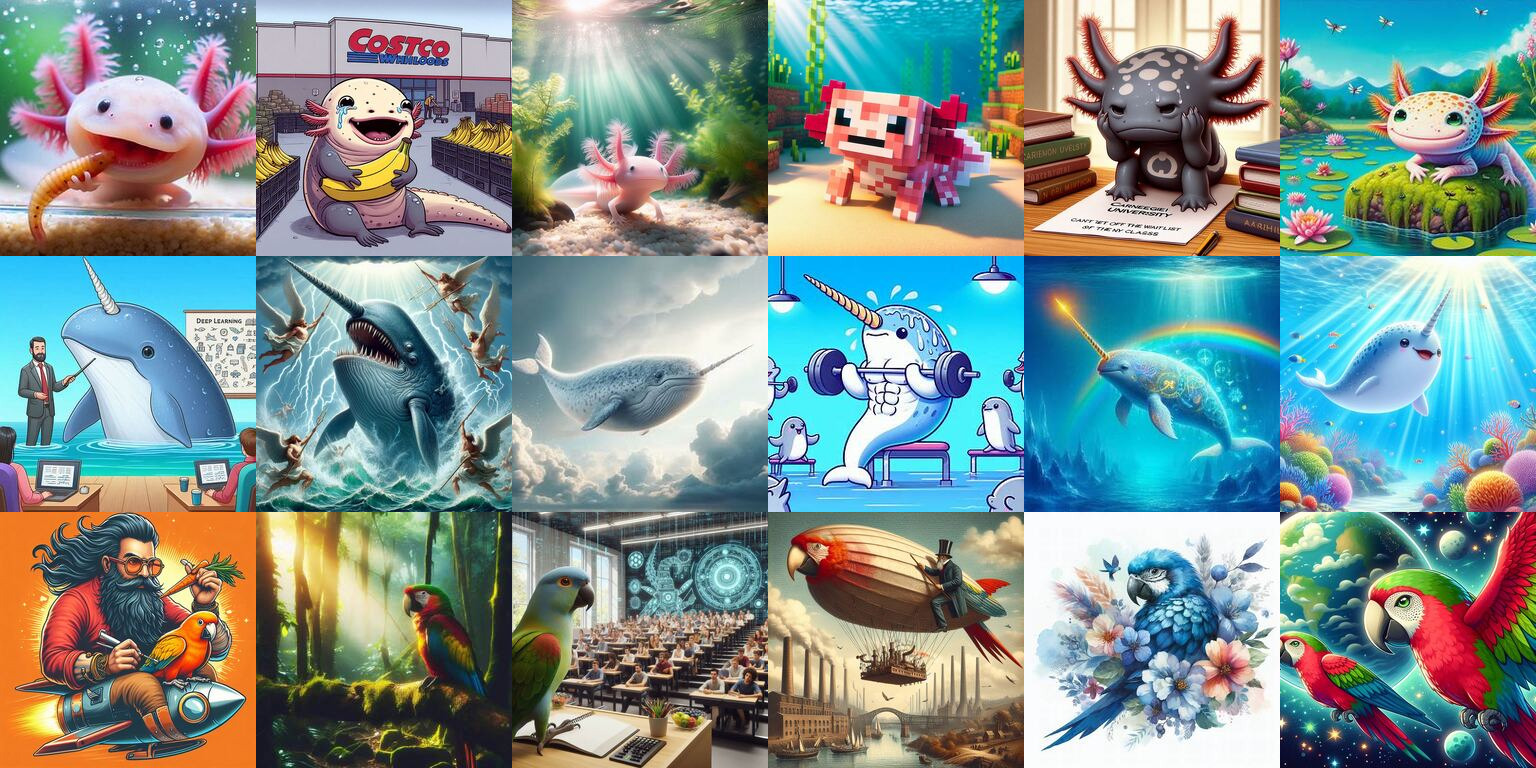
\includegraphics[width=\textwidth]{fig/montage.jpg}
    \caption{Examples images from Parrot/Narwhal/Axolotl dataset.}
    \label{fig:montage}
\end{figure}

\clearpage

\sectionquestion{Image Classification}
\label{sec:image_classification}

In this section, you will augment an image classifier written in PyTorch.

\subsection*{Dataset}

The image classification dataset is hot off the press: Each training example consists of an image created by a text-to-image model and is labeled as one of $\{$parrot, narwhal, axolotl$\}$. The dataset consists of:
\begin{description}
    \item \textbf{ \lstinline{./data/img_train.csv} } The training dataset. Each row corresponds to a training example. There are four columns: 
    \begin{enumerate*}
        \item The \lstinline{image} column provides the relative path to the \lstinline{.jpg} file (e.g. \lstinline{./data/parrot/parrot-0.jpg}). 
        \item The \lstinline{prompt} column contains the prompt that was fed into the text-to-image model to generate the image. 
        \item The \lstinline{label} column is the human readable label (e.g. \lstinline{narwhal}). 
        \item The \lstinline{label_idx} column contains an integer representation of the label (i.e. 0, 1, or 2).
    \end{enumerate*}
    \item \textbf{ \lstinline{./data/img_val.csv} } The identically formatted validation dataset. 
    \item \textbf{ \lstinline{./data/img_test.csv} } The identically formatted test dataset.
    \item \textbf{ \lstinline{./data/parrot/ ./data/narwhal/ ./data/axolotl/} } The three directories containing the respectively labeled raw images.
\end{description}
Examples of the images are shown in Figure \ref{fig:montage}. The data is split roughly so that the training data contains 70\%, the validation data 15\%, and the test data 15\%. 

\subsection*{Starter Code}

The starter code in \lstinline{img_classifier.py} is a fully functional (albeit simple) image classifier based on the PyTorch tutorial. 

\begin{quote}
\begin{description}

\item[Data:] The primary changes are to accommodate the Parrot/Narwhal/Axolotl dataset, intead of FashionMNIST. To accomplish this, we provide the class \lstinline{CsvImageDataset} which is a  \lstinline{torch.utils.data.Dataset}. This class reads in the dataset from a given CSV, optionally applying some transformations to the image. The transformations we use in \lstinline{get_data()} are fairly standard: first we resize so that the smallest side of the image is 256 pixels; next we crop out the centermost 256x256 pixels, then we normalize the red/green/blue channels using the mean and standard deviation from ImageNet. 

\item[Model:] The model in \lstinline{NeuralNetwork} is a simple feed forward neural network with ReLU activations. Its input layer takes the 256x256x3 numbers representing an image as features and maps to a first hidden layer of 512 units. The second hidden layer is also 512 units. The output layer is just 3 units, i.e. equal to the number of labels. 

\item[Training:] Notice that our neural network does not explicitly define a \lstinline{nn.Softmax} layer. The  \lstinline{nn.CrossEntropyLoss} works directly with the logits instead since the probabilities coming out of a softmax might be rather small. During training, we optimize the loss using the stochastic gradient descent algorithm, \lstinline{optim.SGD}.

\item[Evaluation:] At the end of each epoch, the model is evaluated on the train. After training it is evaluated on the test dataset. Afterwards the model is saved to disk (and loaded by way of example) in case you wish to resume training from the saved state, or make predictions with the model on another dataset.
    
\end{description}

\end{quote}

\subsection*{Experiments}

Instrument the existing code with \lstinline{wandb}. First, use \lstinline{wand.init()} to set the project name and store hyperparameters. Next use \lstinline{wandb.log()} to track the loss of each batch and the current number of examples for which we've computed a gradient. Then, in a single call to \lstinline{wandb.log()} at the end of each epoch, track the train accuracy, train loss, test accuracy, test loss, and the current epoch number.

\begin{parts}

\part[3] Run the image classifier with the default hyperparameters. Using \lstinline{wandb}, plot the training loss of each batch vs. the total number of examples seen so far by the optimizer. The loss should be the average loss, taking the average within each batch. Name your run ``neural-the-narwhal''  and include the legend in your graph. 

    \begin{answer_box}[title=,height=8cm, width=15cm]


    \end{answer_box}

\part[3] Report the final train/test accuracy, and the final train/test loss. (You do not need to use \lstinline{wandb} to create this table.)
        
    \begin{answer_box}[title=,height=3cm, width=10cm]
        \begin{center}
            \begin{tabular}{ccc}
                \toprule
                Dataset & Accuracy & Loss \\
                \midrule
                Train & & \\
                Test & & \\
                \bottomrule
            \end{tabular}
        \end{center}
    \end{answer_box}
    

\newpage
\uplevel{The dataset contains a validation set, but the starter code does not use it. Augment \lstinline{img_classifier.py} so that the validation accuracy/loss are computed at the end of each epoch and reported to \lstinline{wandb}.}

\part[4] Plot the train loss and the validation loss on the same plot with the number of epochs on the horizontal axis. The train loss should be averaged over the entire training dataset, and do likewise for the validation loss.

    \begin{answer_box}[title=,height=8cm, width=15cm]

    \end{answer_box}

\part[4] Plot the train accuracy and validation accuracy on the same plot with the number of epochs on the horizontal axis. 

    \begin{answer_box}[title=,height=8cm, width=15cm]
    \end{answer_box}

\newpage
\part Surprisingly, this simple model does seem to be able to learn to distinguish (at least some of) the parrot/narwhal/axolotl images. Perhaps the reason for this success is that the colors of the animals tend to be quite different. Change the sequence of transforms in \lstinline{transform_img = T.Compose([...])} so that it converts the image to a single channel grayscale image using \lstinline{torchvision.transforms.Grayscale}. Be sure to adjust your model to accommodate the new input size! \revert{(Revert back to using color images after this question.)}

\begin{subparts}
    \subpart[3] What is the test accuracy with color images vs. grayscale images? 
        
        \begin{answer_box}[title=,height=3cm, width=10cm]
        \begin{center}
            \begin{tabular}{ccc}
                \toprule
                Dataset & Image Type & Accuracy \\
                \midrule
                Test & Color & \\
                Test & Grayscale & \\
                \bottomrule
            \end{tabular}
        \end{center}
        \end{answer_box}

        
    \subpart[2] Does this support the hypothesis that the classifier wasn't really learning anything besides the color of the animals? 

        \begin{answer_box}[title=,height=3cm, width=\linewidth]
        \end{answer_box}

\end{subparts}

\part[2] Next consider what happens if we work with really tiny images. Resize each image to $(28 \times 28)$ (the standard size of an MNIST digit). What is the test accuracy in this case?  \revert{(Revert back to resizing images to $(256 \times 256)$ after this question.)}

\begin{answer_box}[title=,height=1cm, width=2cm]
\end{answer_box}

\part For the first batch of each of the datasets (train, val, test), on the last epoch only, log each of the images with a caption containing its predicted label as a string (i.e. parrot, narwhal, axolotl) and its true label as a string. Format the caption as ``\lstinline{<predicted label> / <true label>}''. 


\begin{subparts}

    \subpart[2] Show the first batch of the training dataset captioned appropriately on wandb.

        \begin{answer_box}[title=,height=3cm, width=\linewidth]
        \end{answer_box}

\newpage
    \subpart[2] Show the first batch of the validation dataset captioned appropriately on wandb.

        \begin{answer_box}[title=,height=3cm, width=\linewidth]
        \end{answer_box}

    \subpart[2] Show the first batch of the test dataset captioned appropriately on wandb.

        \begin{answer_box}[title=,height=3cm, width=\linewidth]
        \end{answer_box}

    \subpart[2] Pick a few of the images on which the model made an error, and try to explain why it might have had difficult with those images. Answer in just a few sentences.

        \begin{answer_box}[title=,height=3cm, width=\linewidth]
        \end{answer_box}

\end{subparts}


\part Our current optimizer is stochastic gradient descent (\lstinline{torch.optim.SGD}). Change to some other optimizer from \lstinline{torch.optim}\footnote{\url{https://pytorch.org/docs/stable/optim.html}} and adjust the hyperparameters to see if you can achieve better performance than SGD. \emph{If you don't get better performance, you can still receive full credit here.}
\revert{(Revert back to using SGD after this question.)}

\begin{subparts}

    \subpart[2] Report which optimizer and hyperparameters you chose.
    % Which optimizer did you choose and what hyperparameters did you select?

        \begin{answer_box}[title=,height=5cm, width=15cm]
        \end{answer_box}
        
\newpage
    \subpart[3] Then plot the train accuracy and validation accuracy on the same plot with the number of epochs on the horizontal axis. Include a run with SGD and with the new optimizer. Name your runs ``SGD'' and the name of the new optimizer and include the legend. 

        \begin{answer_box}[title=,height=8cm, width=15cm]
        \end{answer_box}

\end{subparts}

\part The model we're using is incredibly simple: a feed-forward neural network with two hidden layers of size 512 units, and ReLU activations. Define a new model that implements the following computation graph:

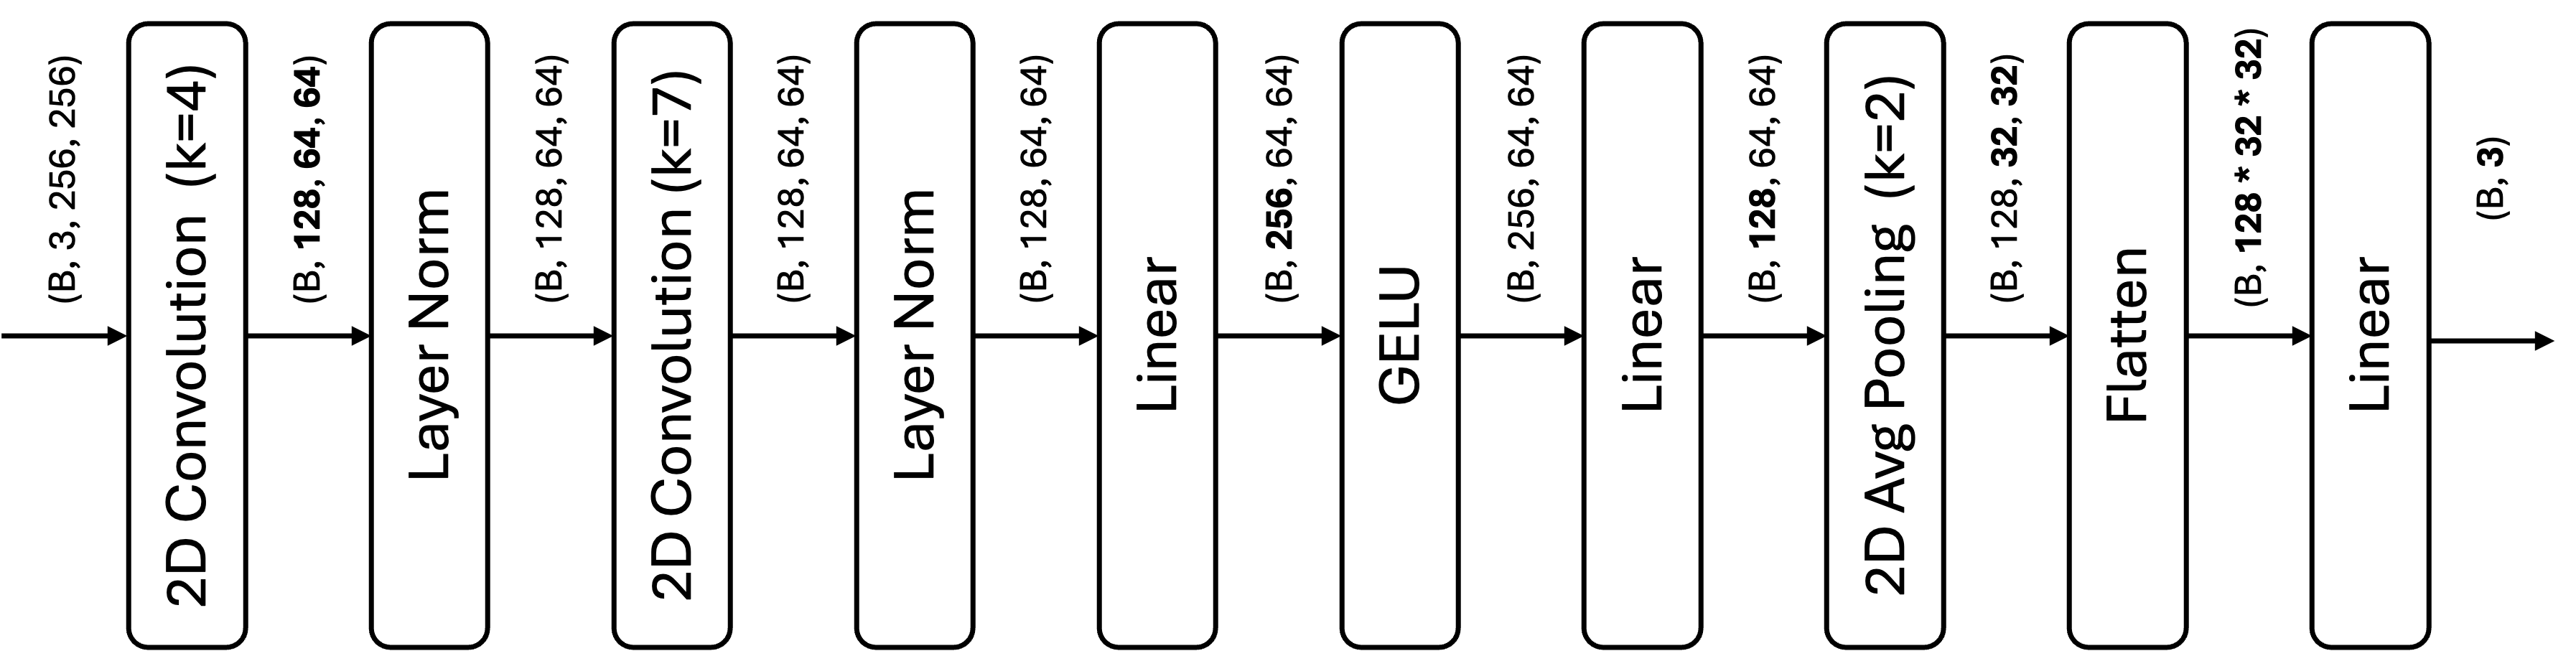
\includegraphics[scale=0.55]{fig/new_model_graph.png}

The tuples denote the dimensions \lstinline{(Batch Size, Channels, Img Height, Img Width)} of the output from the upstream layer and \lstinline{k} denotes the kernel size.

You should review the documentation of \lstinline{torch.nn}\footnote{\url{https://pytorch.org/docs/stable/nn.html}} and select corresponding modules for each layer of the graph. 

Pay special attention to the dimensions in bold that change across layers to determine the correct parameters for each module. There may be more than one valid module or method of implementation for some layers.

\clearpage

\begin{subparts}

    \subpart[1] Report the final train/test accuracy of your new model.

        \begin{answer_box}[title=,height=3cm, width=10cm]
        \begin{center}
            \begin{tabular}{ccc}
                \toprule
                Dataset  & Accuracy \\
                \midrule
                Train  & \\
                Test  & \\
                \bottomrule
            \end{tabular}
        \end{center}
        \end{answer_box}
        
    \subpart[4] With \lstinline{wandb}, plot the train accuracy and validation accuracy on the same plot with the number of epochs on the horizontal axis. Include a run with the original model and a run with your new model. Name your runs ``new-model'' and ``base-model'' and include a legend. 
        
        \begin{answer_box}[title=,height=8cm, width=15cm]
        \end{answer_box}


    \subpart[2] How many parameters were in your original model and new model? (Refer to the recitation handout for how to calculate these numbers.)

        \begin{answer_box}[title=Original model,height=2cm, width=4cm]
        \end{answer_box}
        
        \begin{answer_box}[title=New model,height=2cm, width=4cm]
        \end{answer_box}

\clearpage

    \subpart[2] Did your new model perform better or worse on the test set than the original model? What factors might explain the differences in accuracy you observed between the models?

        \begin{answer_box}[title=,height=8cm, width=15cm]
        \end{answer_box}

\end{subparts}

\end{parts}

\clearpage

\begin{table}[b]
    {\small 
    \begin{tabular}{p{0.2\linewidth}p{0.4\linewidth}p{0.4\linewidth}}
        \toprule
        Title & Real Article & Fake Article 
        \\
        \midrule
        Vice Mayor of Wenzhou City Chen Yingxu and his delegation visited Ruian Middle School to investigate mental health education work
        &
        On November 27, 2023, Wenzhou Deputy Mayor Chen Yingxu and his delegation visited Ruian Middle School for investigation and guidance, and learned about the school’s campus safety, mental health education and other work...
        &
        Wenzhou City, China - [Date]
        In a proactive move towards enhancing the mental well-being of students, Vice Mayor Chen Yingxu led a delegation to Ruian Middle School to delve into the intricacies of mental health education...
        \\
        \midrule 
        Bensalem Letter Carrier Honored For 43-Year Career 
        & 
        BENSALEM TOWNSHIP, PA —He was her mailman for 30 years.
        Every day, Debbie McBreen would see the man "who always had a smile on his face" —U.S. Postal Service letter carrier Kyle Livesay.
        "He was amazing, so friendly. He is just a wonderful person and an excellent man," said McBreen...
        &
        In a heartwarming ceremony held at the Bensalem Post Office, the community came together to celebrate the remarkable career of Mr. John Anderson, a dedicated letter carrier who has faithfully served the residents of Bensalem for an impressive 43 years...
        \\
        \midrule
        No straight drive today as traffic to be diverted for T20I
        &
        Indore: As the city gears up for the much-anticipated T20I cricket match between India and Afghanistan on Sunday, Indore police released a traffic diversion plan to ensure a smooth commute during the match. DCP traffic Manish Agarwal said special arrangements have been made to ensure zero traffic block incidents on Sunday...
        &
        In anticipation of the throngs of cricket enthusiasts expected to flood the city for today's exciting Twenty20 International (T20I) match, city officials have announced a comprehensive traffic diversion plan. The match, set to be a showdown between two of the world's leading cricket teams...
        \\
        \bottomrule
    \end{tabular}
    }
    \caption{Examples of article snippets from the dataset.}
    \label{tab:txt_examples}
\end{table}


\clearpage

\sectionquestion{Text Classification}
\label{sec:text_classification}

In this section, you will augment a text classifier written in PyTorch.

\subsection*{Dataset}

\begin{notebox}
    Note that the news articles, real and fake, in this dataset have not been filtered. Please take care when reading any of the data.
\end{notebox}

The text classification dataset consists of news articles, real and fake. The real articles were selected from news outlets around the world, with an emphasis on small-town local news. Each fake article was generated by a large language model with a prompt that included the title of the corresponding real news article.

The dataset is contained in three \lstinline{.csv} files in UTF-8 encoding.
\begin{center}
    \lstinline{./data/txt_train.csv} \quad 
    \lstinline{./data/txt_val.csv} \quad 
    \lstinline{./data/txt_test.csv} 
\end{center}
Each one is identically formatted with one example per row. There are four columns:
    \begin{enumerate}
        \item The \lstinline{article} column contains the text of the news article. The title of the article is prepended as the first line of this article text.
        \item The \lstinline{source} column differs for real/fake examples. For a real example, it contains the URL of a real article. For a fake example, it contains the prompt that was fed into the LLM to generate the article. 
        \item The \lstinline{label} column is the human readable label (i.e. \lstinline{real} or \lstinline{fake}). 
        \item The \lstinline{label_idx} column contains an integer representation of the label (i.e. 0 or 1).
    \end{enumerate}
Examples of the news articles are shown in Table \ref{tab:txt_examples}. The data is split roughly so that the training data contains 70\%, the validation data 15\%, and the test data 15\%. Each of the train/val/test CSV files are sorted so that the pairs of real/fake news articles are adjacent rows.

\subsection*{Starter Code}

The starter code in \lstinline{txt_classifier.py} is a fully functional (albeit simple) text classifier based on the PyTorch tutorial for text classification. Before you continue, you should read this tutorial as it differs from the main PyTorch tutorial.
\begin{center}
{\small
\url{https://pytorch.org/tutorials/beginner/text_sentiment_ngrams_tutorial.html}
}
\end{center}

\begin{quote}
\begin{description}

\item[Data:] The dataset for this section is similar in form to that from the tutorial. The starter code provides the class \lstinline{CsvTextDataset} which is a \lstinline{torch.utils.data.Dataset}. This class reads in the dataset from a given CSV, optionally applying some transformations to the text. 
%
We read the training dataset twice: the first time we tokenize the text but do \emph{not} numericalize the tokens in order to build a vocabulary (i.e. a mapping of tokens to integers). The second reading of the training data then proceeds with numericalization. Each article is also truncated to some maximum number of tokens.
%
The \lstinline{DataLoader} uses a \lstinline{collate_fn}, which is simply a callable (or function) that is applied to each batch. You will explore the behavior of our \lstinline{PadSequence} in the questions below.

\item[Model:] The \lstinline{TextClassificationModel} consists of just two layers and is detailed in the text classification tutorial. 

\item[Training:] The training process proceeds as usual: optimizing a cross entropy objective with SGD. 

\item[Evaluation:] The model periodically evaluates on the train and validation set, and finally on the test set. 
    
\end{description}
    
\end{quote}

\subsection*{Experiments}

(You are welcome, but not required, to instrument the code with \lstinline{wandb}.)
 
\begin{parts}

\part[3] Generate a histogram of the lengths of the news articles after truncating with \lstinline{MAX_LEN} but before padding the sequence in the training dataset. You can do this however you'd like. (One option is to use  \lstinline{wandb}. If doing so, you should follow the ``Histograms in Summary'' instructions from \href{https://docs.wandb.ai/guides/track/log/media#histograms}{here}. You will need to click on the run, then on its Overview tab, and then scroll to the bottom to find it.)

    \begin{answer_box}[title=,height=5cm, width=15cm]
    \end{answer_box}

\part[3] Run the code three times and report the validation and test accuracies. (You can easily create such a table on the ``Runs'' tab of \lstinline{wandb} if these are logged.) 

    \begin{answer_box}[title=,height=3.5cm, width=10cm]
    \begin{center}
    \begin{tabular}{ccc}
        \toprule
        & Val. Acc. & Test Acc. \\
        \midrule
        Run 1 & & \\
        Run 2 & & \\
        Run 3 & & \\
        \bottomrule
    \end{tabular}        
    \end{center}
    \end{answer_box}


\part[2] Switch the optimizer to \lstinline{torch.optim.Adam}\footnote{\url{https://pytorch.org/docs/stable/generated/torch.optim.Adam.html}}, then run the code three times and report the validation and test accuracies. \revert{(Do NOT revert this change, but use Adam for future questions as well.)}
    
    \begin{answer_box}[title=,height=3.5cm, width=10cm]
    \begin{tabular}{ccc}
        \toprule
        & Val. Acc. & Test Acc. \\
        \midrule
        Run 1 & & \\
        Run 2 & & \\
        Run 3 & & \\
        \bottomrule
    \end{tabular}      
    \end{answer_box}


\part Carefully read the documentation for \lstinline{nn.Embedding}\footnote{\url{https://pytorch.org/docs/stable/generated/torch.nn.Embedding.html}} and then \lstinline{nn.EmbeddingBag}\footnote{\url{https://pytorch.org/docs/stable/generated/torch.nn.EmbeddingBag.html}} paying close attention to the \lstinline{padding_idx} parameter and the associated examples. Next read the code for \lstinline{PadSequence} in \lstinline{txt_classifier.py} so that you understand what it is doing. 
\revert{(After this question, revert back any changes you made in the course of answering it.)}


\begin{subparts}

    \subpart[1] Change the code so that the \lstinline{collate_fn} parameter is not passed to the DataLoaders. What error is reported? 
    \begin{answer_box}[title=,height=3cm, width=15cm]
    \end{answer_box}
    
    \subpart[2] Why is this considered an error?
    \begin{answer_box}[title=,height=3cm, width=15cm]
    \end{answer_box}
    
    \subpart[1] Now change the batch size to be 1 (instead of 8). What error is reported? 
    \begin{answer_box}[title=,height=2.5cm, width=15cm]
    \end{answer_box}

    \subpart[2] Why is this new error happening?
    \begin{answer_box}[title=,height=3cm, width=15cm]
    \end{answer_box}
    
\end{subparts}

\clearpage
\part Replace the simple \lstinline{TextClassificationModel} with an LSTM-based classifier. This can be any architecture of your choosing, so long as it uses \lstinline{torch.nn.LSTM}\footnote{\url{https://pytorch.org/docs/stable/generated/torch.nn.LSTM.html}} in some reasonable way (e.g. unidirectional LSTM, bidirectional LSTM, deep LSTM). For those new to LSTMs: use the code presented in the HW0 recitation. Please read through the PyTorch documentations for \href{https://pytorch.org/tutorials/beginner/nlp/sequence_models_tutorial.html}{sequential models} and \href{https://pytorch.org/docs/stable/generated/torch.nn.LSTM.html}{LSTM} for more examples and clarifications on implementation details. 

\begin{subparts}

    \subpart[2] In math, pseudocode, or a computation graph, describe the structure of your new model.
    \begin{answer_box}[title=,height=7cm, width=15cm]
    \end{answer_box}

    \subpart[4] Plot the train and validation accuracies of your model against the original model. Your results do not have to be better than the original model.  

    \begin{answer_box}[title=,height=8cm, width=15cm]
    \end{answer_box}

\clearpage

    \subpart[2] Describe any differences in performance between your model and the original model. In a few sentences, discuss why your model worked better or worse than the original model. 

    \begin{answer_box}[title=,height=5cm, width=15cm]
    \end{answer_box}
    
\end{subparts}


\part[2] Look through a few of the real/fake news article pairs. In a few sentences, speculate on how the model is able to train successfully.

    \begin{answer_box}[title=,height=5cm, width=15cm]
    \end{answer_box}

\end{parts}

\clearpage

\sectionquestion{Code Upload}

\begin{parts}

\part[0] Did you upload your code to the appropriate programming slot on Gradescope? \\
\emph{Hint:} The correct answer is `yes'.

    \begin{checkboxes}
     \choice Yes 
     \choice No
    \end{checkboxes}

For HW0, you should upload \emph{two} files: \lstinline{img_classifier.py} and \lstinline{txt_classifier.py} that include all your interesting new changes to the code.

\end{parts}

\newpage
\sectionquestion{Collaboration Questions}

\begin{parts}

\uplevel{After you have completed all other components of this assignment, report your answers to these questions regarding the collaboration policy. Details of the policy can be found in the syllabus.}

    \part[1] Did you collaborate with anyone on this assignment? If so, list their name or Andrew ID and which problems you worked together on.

        \begin{answer_box}[title=,height=3cm, width=15cm]
        \end{answer_box}

    
    \part[1] Did you find or come across code that implements any part of this assignment? If so, include full details.
        \begin{answer_box}[title=,height=3cm, width=15cm]
        \end{answer_box}
\end{parts}
\end{questions}


\end{document}
